\section{Import mask protocol}
\label{app:importMask}%a091
Protocol designed to import a mask in \scipion from a file of user's computer. Modifying the size of a previous mask is possible simply by changing the mask's sampling rate.
   
 \begin{itemize}
        \item Requirements to run this protocol and visualize results:
                \begin{itemize}
                    \item \scipion plugin: \ttt{scipion-em}
                \end{itemize}
        \item \scipion menu:
            It does not appear in \ttt{Model building} view.
            Press \scommand{Ctrl} + \scommand{f} and the pop up window to search a protocol will be opened ((\ffigure{fig:app_protocol_assign_orig_and_sampling} (A)). Write any word related with the title of the protocol that you are looking for in the \ttt{Search} box. In this particular case we have written \ttt{mask}. Several protocols have been found related with this search word. Select the first one dessigned for the purpose that we are interested in (\ttt{pwem - import mask}).
  
        \item Protocol form parameters (\ffigure{fig:app_protocol_assign_orig_and_sampling} (B)):
  
            \begin{figure}[H]
                \centering 
                \captionsetup{width=.7\linewidth} 
                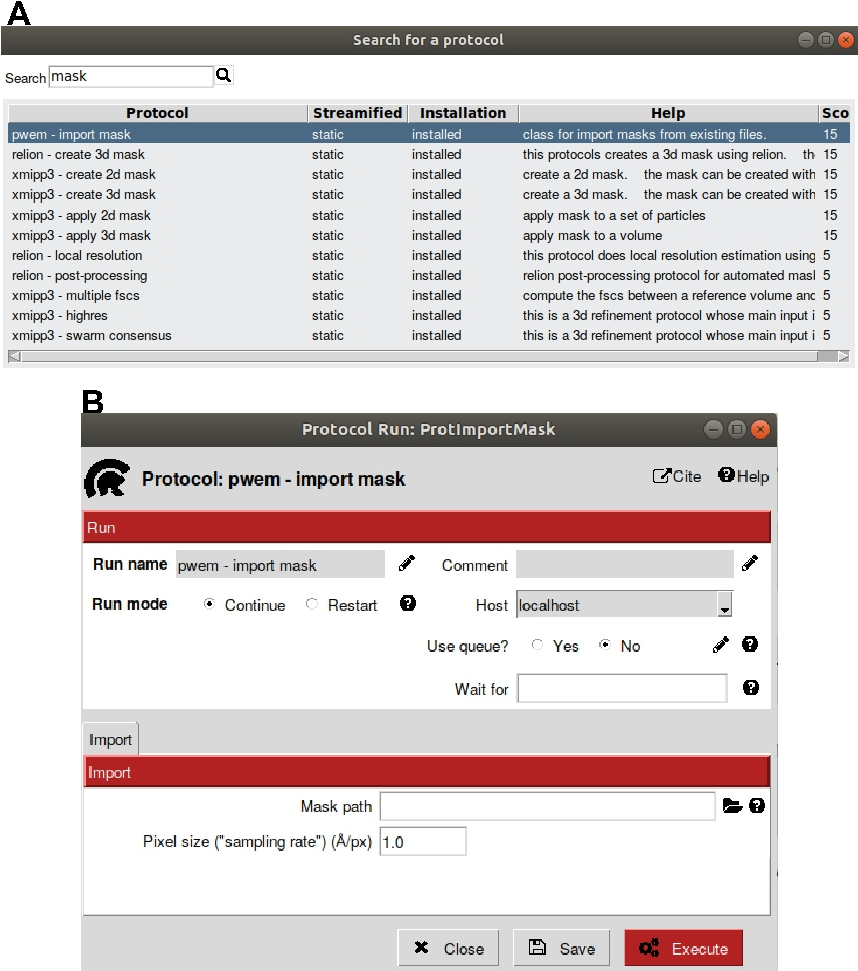
\includegraphics[width=0.90\textwidth]{Images_appendix/Fig304.pdf}
                \caption{A. Protocol \scommand{import mask}. A: Window to search the protocol. B: Protocol form.}
                \label{fig:app_protocol_import_mask}
            \end{figure}
  

        \item \ttt{Input} section
  

            \begin{itemize}
                \item \ttt{Mask path}: Open the browser on the right to select in your computer the path to the previously saved mask.
                \item \ttt{Pixel size (``sampling rate'')} (\AA/px): Write the new sampling rate rate value in the box. 
            \end{itemize}

  
        \item Protocol execution:
  
            Adding specific mask label is recommended in \ttt{Run name} section, at the form top. To add the label, open the protocol form, press the pencil symbol at the right side of \ttt{Run name} box, complete the label in the new opened window, press OK, and finally, close the protocol. This label will be shown in the output summary content (see below). If you want to run again this protocol, do not forget to set to \ttt{Restart} the \ttt{Run mode}.\\
            Press the \ttt{Execute} red button at the form bottom.
  

        \item Visualization of protocol results:
  
            After executing the protocol, press \ttt{Analyze Results} and $ShowJ$, the default \scipion viewer, will allow you to visualize the \ttt{slices} window of the mask  (\ffigure{fig:create3Dmask_2}). The $ShowJ$ window menu (\ttt{File -> Open with ChimeraX}) allows to open the selected map in $ChimeraX$ graphics window.
   
            \begin{itemize}
                \item \ttt{slices}: $ShowJ$
                
                \url{https://github.com/I2PC/scipion/wiki/ShowJ}

            \end{itemize}
   
        \item Summary content:
    
            \begin{itemize}
            \item Protocol output (below \scipion framework):\\ \ttt{pwem - import mask -> ouputMask};\\ \ttt{VolumeMask (x, y, and z dimensions, sampling rate)}.
            \item \ttt{SUMMARY} box:\\\ttt{Mask file imported from}: The specific selected path to the mask in your computer should appear here.
            \end{itemize}
  
  \end{itemize}
